\chapter{Innovations- und Transformationsprozesse}
Dieses Kapitel analysiert die Einflüsse aus den Rahmenbedingungen auf Veränderungsprozesse von Organisationen und trägt kontinuierlich zur Findung der Ursachen der genannten Probleme und Ansätze für ihre Lösung bei. Der \emph{Design-Thinking} Prozess wird hierbei als iterative Gestaltungsmethode für Ideen, Prototypen und kontinuierlicher Evaluierung verwendet. Daher bauen die nachfolgenden Abschnitte aufeinander auf und sollen somit zu einer kontinuierlichen Verbesserung beitragen und in ihrer letzten Ebene ausgeliefert werden.

\section{Einflüsse und Kräfte der Innovation}
\citet{Ganswindt2006} und \citet{Koch2016} identifizieren bereits, dass das \ac{ITM} nicht in der Lage ist die Maßnahmen für eine Transformation zu priorisieren.
Die gegenseitigen Einflüsse sind ineinander verwachsen und es werden häufig zu erst die Symptome bekämpft (Anh.\ref{appendix:docker}, Kap. \ref{jenkins:skalierung}).

\paragraph{Komponenten der Legacy-IT}
\label{einschr:assets}
Aufgrund dieser Verwachsungen wird in der folgenden Auflistung eine grobe Lokalisierung und Zusammenfassung vorgenommen:
\begin{itemize}
    \item \textbf{Organisation:} tiefe Silos \cite{Gupta:2017}, Schatten-IT \cite{recht/Bornemann2018}, Abhängigkeiten, Handlungsunfähigkeit, Redundanzen, mangelnde Priorisierung, langsame Prozesse
    \item \textbf{IT-Architektur:} Komplexität \cite{Brockhoff2006}, steigende Anforderungen \cite{Brockhoff2006}, Kosten für Eigenentwicklung \cite{Gupta:2017}, Proprietäre Anwendungen \cite{Bussmann2006}, veraltete Systeme, mangelnde Skalierbarkeit, Legacy-IT
    \item \textbf{Regulatorik:} \ac{IDV} Katalogisierung\cite{recht/Bornemann2018}, fehlende Präzisierung, steigende Anforderungen
\end{itemize}

Es fällt auf, dass es erheblich schwierig ist die Einschränkungen für eine Transformation zu faktorisieren. Es ist weitaus einfacher direkte Gegenmaßnahmen auf die beobachtete Einschränkung vorzuschlagen oder antreibende Eigenschaften wie Agilität zu fordern. Daher werden die antreibenden Faktoren nachfolgend betrachtet.

\subsection{Innovationsverlauf als disruptive S-Kurven}
\citet[Kap. 2.2]{Alt2017} erklären die Abläufe einer Innovation. Die Abbildung \cite[Abb. 2.1]{Alt2017} beschreibt einen Innovationsverlauf als eine \emph{S-Kurve} \cite{Ganswindt2006}, die in Folge mehrerer aneinander gereihte Innovationen gesamtheitlich betrachtet einen disruptiven Verlauf mit Sprüngen zeigen. Darunter liegt die Adaptionskurve, die als die Ableitung der Innovationskurve erscheint. 

Einschränkenden Faktoren, die in Banken beobachtet werden, könnten auf dem ersten Blick als Faktor der Adaptionskurve in \cite[Abb. 2.1]{Alt2017} zugeordnet werden und die Adaption beschränken. Demgegenüber stehen die zu erarbeitenden Gegenmaßnahmen zur Lösung des Problems. Instinktiv können einige Einschränkungen, die eine Eigenschaft darstellen negiert werden. Komplexität wird beispielsweise zu Nachvollziehbarkeit. Die Meisten benannten Einschränkungen sind jedoch keine Effekte, die die Innovationskraft \cite{Ganswindt2006} beeinflussen. Sie beeinflussen aber die bevorstehende Transformation. 
\medskip
\\
Innovationen unterliegen kreativen Prozessen \cite[S.14]{Alt2017}, weswegen eine kreative Methode sich für ihr Verständnis eignen könnte. Gerade der \emph{Design-Thinking} Prozess sieht die iterative Gestaltung und Evaluierung von Prototypen vor. Dadurch können Zusammenhönge untersucht werden und der Lösungsansatz kann ständig angepasst werden.
\medskip
\\
In folge wurde Abbildung \ref{fig:digit-trans} in mehreren Iterationen der Syntheseschritte \enquote{ideate-prototype-testing} aus dem Design-Thinking Prozess (Kap. \ref{def-design-thinking}) mithilfe von den Punkten aus \cite[S. 14]{Alt2017} und dem erarbeiteten Rahmen in Kap. \ref{ch:background} generiert.
%

\begin{figure}[htbp]
 \centering
 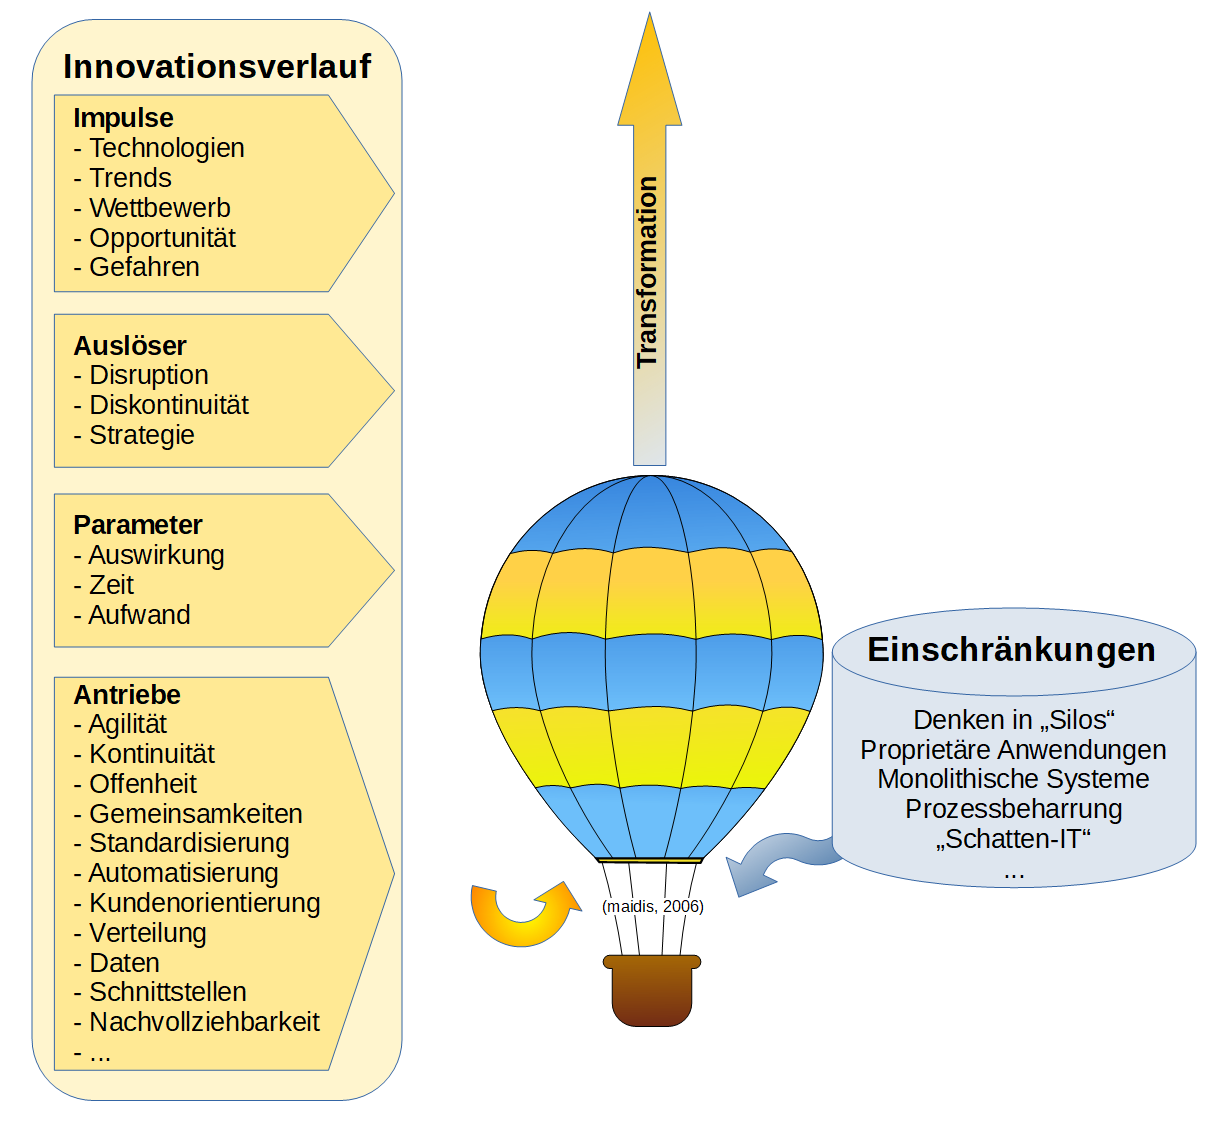
\includegraphics[width=1.0\textwidth]{gfx/digital-transformation-lifecycle-by-selim3.PNG}
 \caption{Innovationsverlauf und Regelung einer Transformation (Quelle: eigene Darstellung, Heißluftballon von \citet{maidis_2006})\label{fig:digit-trans}
 }
\end{figure}
%
\paragraph{Beschreibung Innovationsverlauf}
Innovationen und Innovationsverläufe sind voneinander zu unterscheiden. Die Innovation ist das Neue, während ein Innovationsverläuf als ihr Einschlag in die Organisation oder Gesellschaft gesehen werden kann. Ein Innovationsprozess wäre eine gezielte Regelung oder Steuerung nach dem Einschlag.

Ein Innovationsprozess setzt daher einen Auslöser voraus und beginnt mit \emph{Sharing} (Abb. \ref{fig:devops}).

Dieser Einschlag kann kontrolliert anhand einer Strategie in die Umgebung gesetzt werden oder durch äußere Einflüsse unkontrolliert in Form einer Disruption oder Diskontinuität \cite{Fernandez:2020} des aktuellen Zustands eindringen.

Das Eindringen der Disruption wird in  als Angriff gesehen, was für ein IT-Risikomanagement berechtigt wäre.
Diskontinuität könnten dagegen als Ausstoß gesehen werden.
\medskip
\\
Sie Zeigen sich als Impuls, die Bewegungen anstoßen.
Weitergeführt werden in (Abb. \ref{fig:digit-trans}) die Antriebe der Innovation beschrieben. Diese steigern die Innovationskraft und wirken gegen die Widerstände, genannt Einschränkungen. Die Antriebe sind hierbei in Form von Anforderungen nur ein Soll-Zustand der Organisation. Sie ermitteln sich aus der Last der Legacy-IT. 
%
\paragraph{Ursprung der Idee}
Der Begriff der antreibenden und einschränkenden Faktoren generierte in Zusammenhang mit dem Transformationsziel der heutigen IT-Architekturen hin zu einer Cloud-Architektur die Idee von einem Heißluftballon als Metapher für die sich transformierende Organisation.

\paragraph{Auswirkung auf die Transformation}

Wird das ganze mit einem entsprechenden physikalischen Zusammenhang betrachtet scheint es sofort ersichtlich, dass geplante Transformationen mit Gegengewichte belastet werden. Der Arbeitsaufwand für die Transformation steigt exponentiell, je schwergewichtiger die Organisation ist. Veränderungsprozesse oder Transformationen können nicht mit linearen Metriken geplant werden. Daher entsteht auch das Problem von exponierenden Budgets in Anpassungsprojekten.
\medskip
\\
Um eine Transformation zu planen reichen Aufwände und Zeitrahmen nicht aus. Die Transformation bedingt eine Innovationskraft, die sich aus der Wechselwirkung zwischen vorhandenem Antrieb und Einschränkungen ergibt. Sind genügend Antriebe vorhanden und wenig Last kann auch Traktion entstehen.
\medskip
\\
Die Maßnahmen der Legacy-IT in Banken richten sich nach den falschen Metriken und Zielen. Ziel ist es nicht eine Arbeit hinter sich zu bringen. Technologiesprünge werden frequentierter und Strecke immer länger.
Die aktuellen Maßnahmen richten sich nur nach den Einschränkungen. Diese sind erstmal nicht relevant, da sie sich nicht selbst überwinden können. Für die Innovationskraft spielt der materielle Zusammenhang keine Rolle.

\paragraph{Bildlich weitergeführt}
Die Analogie eines Heißluftballon für die Regelung der Transformation kann folgendermaßen fortgeführt werden:

Die Kräfte im Ballon sind dynamisch und bewegen mit genug Antrieb ein statisches Abbild der Organisation, welcher im Korb des Heißluftballon liegt und einen Zustand der Organisation beschreibt. Der Korb ist in sich geschlossen und beinhaltet den Ablauf und Aufbau des Kerngeschäfts. Dieser trägt zu ihrer Unterstützung viele weitere Funktionen mit, die jeweils die Bewegung der Organisation durch ihre Last exponentiell einschränken. Die Bewegung kann auf zwei Arten beschleunigt werden. Der Antrieb wird erhöht oder ein Teil der Einschränkungen abgeworfen. Sie kann nicht gesteuert werden, wodurch externe Einflüsse sie stark beeinflussen können. Das Objekt gleitet hierbei im Strom einfach mit.
\medskip
\\
\paragraph{Lehren aus Docker}
Ein statisches Abbild mit Prozessbeschreibungen und Ausführung als eine in sich geschlossene Einheit ist aus der Virtualisierung von Systemen bekannt. Mit zunehmender Automatisierung der Geschäftsprozesse finden sich auch zunehmende Gemeinsamkeiten zwischen Organisationen und IT-Systemen. 

Best-Practices zur Beschreibung von Images mit Docker könnten als Inspiration für Organisationen dienen. Besonders das Minimalisieren von Images durch schlanke und funktionale Ebenen sowie Kubernetes zur flexiblen Skalierung und Orchestrierung von ganzen System könnten als Idee für eine flexible und skalierbare Orchestrierung von Veränderungen für die Organisation dienen, um ihre Transformationsfähigkeit zu erhöhen. Der schmerzvolle Rollout bei wesentlichen Veränderungen in großen Organisationen könnte in eine vollautomatisierte Orchestrierung umgewandelt werden.
Agile Prinzipien in der Kultur wären das Docker und ein neues effektives Change-Management das Kubernetes des Managements.

Nach einer solchen zukünftigen Entwicklung wäre die Idee von \emph{Development as a Service} \ref{Disruption:DaaS} mit entsprechenden eingespielten Abläufen durchaus realistisch. Andere disruptive Entwicklungen sind auch nicht ausgeschlossen. Umso wichtiger ist es einen Weg zu finden die Digitale Transformation zu beherrschen.

%
%
%
%


\section{Frage an das Management: Change oder Run?}
\paragraph{Transformationsfähigkeit als Prinzip}
Abb. \ref{fig:digit-trans} stellt für den Umgang mit wesentlichen Veränderungen ein erstes Prototyp dar. Die Abbildung beschreibt möglicherweise einen Zustand vor einer bevorstehenden Transformation.

Daher dient sie als Grundlage, um Anforderungen für einen innovativen Soll-Zustand zu simulieren. Ein innovativer Soll-Zustand der Organisation würde eine höchstmögliche Transformationsfähigkeit bedeuten.
\medskip
\\
Gleichzeitig zeigt sie, dass mit Anforderungen und Kenntnissen über Einschränkungen eine bevorstehende Transformation nur geregelt werden kann und die Richtung nicht absehbar ist. Gas geben ohne zu lenken ist für FinTechs und Start-ups kein großes Problem, da aufgrund ihrer kleinen Größe die Auswirkungen von Veränderungen einfacher analysiert werden können.

Für die größeren, etablierten Institute gilt ein erhöhter Schutzbedarf \cite{recht/Bornemann2018} und dadurch zusätzliche Maßnahmen für die Kontrolle von operationellen Risiken \cite{MaRisk:2017, BAIT:2018}. Diese müssen gezwungenermaßen sich neu ausrichten \citet{Bussmann2006, Gupta:2017}, indem sie ihre hohe Masse in Bewegung versetzen. Analog impliziert es eine Unkontrollierbarkeit von möglichen Problemen und Risiken.
\medskip
\\
\citet[11.4.1]{Koch2016} fordern für ein Management der Transformation:
\begin{quote}
    \enquote{Erstens ist zu akzeptieren, dass der
Transformationsprozess nicht im Kontext eines einmaligen begrenzten Projektes vollzogen
werden kann. Vielmehr bedarf es einer langfristigen Initiative, damit die notwendigen
Fähigkeiten entwickelt werden können. Zweitens darf die Transformation nicht als rein
technologische Initiative interpretiert werden.}
\end{quote}

Die Entwicklung von skalierbaren und flexiblen Systemen für die \ac{SEU} von Banken setzt wesentliche Veränderungen in der IT-Architektur, Prozesse und Organisation eines Instituts voraus. Erfolgen diese nicht werden umfangreiche Anpassungen der verwendeter Standardsoftware und Abänderungen von gängigen Lösungen bedingt \ref{grundlagen:ci-in-banken}.
\medskip
\\
In folge dessen sind die Veränderungsprozesse selbst zu optimieren und die Einschränkungen hierfür zu eliminieren. Kontinuierliche Veränderungen setzen kontinuierliche Prozesse voraus (Abb. \ref{fig:devops}). Standards in der Softwareentwicklung sind agil und verändern sich ständig. Eine flexible IT-Architektur ist erforderlich, um sich diesen Veränderungen anzupassen \cite{Bussmann2006}.

\paragraph{Errichtung von Anlagen}
\label{anlagen:capabilities}
Aus Sicht der Entwicklung und Beteiligten an Change-Prozessen könnte bezüglich der Einschränkungen auf die Regulatorik oder Betrieb verwiesen werden.

Dagegen spricht aus Sicht des Betriebs, dass Change-Prozesse zuerst sich selbst zu optimieren haben und dadurch die richtigen Prioritäten setzen, bevor sie den ohnehin konservativen Betrieb optimieren. Die Skalierbarkeit und Flexibilität der IT-Architektur sollte nicht aufgrund ihrer Symptome gefordert werden, sondern als eine Anlage\footnote{vgl. \enquote{capabilities} in \cite{Koch2016}}, um weitere Innovationen zu fördern.
\medskip
\\
Möglich wäre eine Strategie, in der Entwickler und Geschäftsleitung eng zusammenarbeiten.
Beim Durchleuchten der Einschränkungen aus verschiedenen Perspektiven fällt auf, dass die konservative Haltung des IT-Betriebs und der Regulatorik eine valide Berechtigung, gerade im Finanzwesen hat. Die Anforderungen selbst sind trotzdem flexibel gestaltet und bieten einen Ermessensspielraum. 

\paragraph{Gestaltungsmethoden für IT-Management}
Neben externe Auslöser von Innovation, die Unternehmen aufgrund von Disruption und Diskontinuität zu Veränderungen zwingen \cite{Gupta:2017, Fernandez:2020} existiert die IT-Strategie als interner Auslöser \cite{BAIT:2018, Alt2017}, dessen Verantwortung in erster Linie der Geschäftsleitung unterliegt \cite{BAIT:2018}. Daher sollten zu erst die Veränderungsprozesse optimiert werden. Eine klare IT-Strategie optimiert sich selbst bevor Forderungen gestellt werden. Dies wird durch Gestaltungsmethoden wie \emph{Design-Thinking} hervorgehoben, indem sie die Quellen zu fremden Problemen zuerst auf sich selbst richten \cite{yüksel:digit}. Gestaltungsmethoden wie Design-Thinking werden gerade für Innovationsprozesse und für das \ac{ITM} empfohlen \cite{Alt2017, Koch2016}. Zudem sollte die in \citet[AT 8.2]{MaRisk:2017} geforderte Analyse und Beteiligung bei wesentlichen Veränderungen schon in den Gestaltungsprozessen stattfinden \cite{Dorschel2018}. Eine Mitgestaltung nach agilen Methoden (Abb. \ref{fig:devops}) ist auch im IT- und Risikomanagement erforderlich, um effiziente Abläufe und Maßnahmen zu schaffen.

\section{Forderung eines effektiven Veränderungsmanagements}
Für die Vorhersehbarkeit von Auswirkungen ist ein kontrollierter Umgang mit Veränderungsprozessen erfordert. Um wesentliche Veränderungen kontinuierlich zu ermöglichen muss die Analyse ihrer Auswirkungen \cite{MaRisk:2017} ebenfalls effektiv sein. Die Vorhersehbarkeit der Auswirkungen von Veränderung sollte nicht nur aufgrund der Regulatorik erfüllt werden. Sie ist als eine Voraussetzung für eine klare Sicht und Zielorientierung für die Transformation anzustreben.
\medskip
\\
Ein effektives Veränderungsmanagement hat das Ziel einen Zustand der höchstmöglichen Transformationsfähigkeit zu erreichen. Hierfür ist ein grundlegend innovatives Paradigma vonnöten. 

\paragraph{Innovativer Soll-Zustand der Kultur}
Die innovative Soll-Kultur (Abb. \ref{fig:digit-trans}, Antriebe) impliziert hierbei Qualitätsansprüche für die Ergebnisse von Innovationsprozessen.

Die Qualitätsansprüche sind Gegenmittel die einschränkenden Faktoren für Veränderung.
Sie dienen daher als Grundlage, um nach einer Kultur zu streben, die sich Transformationsfähigkeit als Prinzip setzt.

Nach \citet[S.30]{Bussmann2006} ist eine kontinuierliche Justierung für den Unternehmenserfolg wichtig. Als eine der Schwierigkeiten nennt er ein effektives Management der Veränderungsprozesse.
\medskip
\\
Diese Schwierigkeit hat sich in Banken bis heute noch bewährt.
Daher wird zum Prototyp aus Abb. \ref{fig:digit-trans} ein erweitertes Modell bedingt. Für den Umgang mit kontinuierlichen Veränderungen erfordert es effiziente kontinuierliche Veränderungsprozesse.
Damit sollen bevorstehende und unvermeidbare Transformationen der Organisation kontrollierbar stattfinden.
Die Frage zu einem Umgang mit kontinuierlichen Veränderungen betrifft das Veränderungsmanagement.
\medskip
\\
\citet[S. 184f]{Koch2016} ordnen das Veränderungsmanagement zu den wichtigsten Anforderungen an ein zukünftiges Paradigma der IT-Organisation. Das bisherige Modell \emph{Plan-Build-Run} ersetzen sie mit einem neuen Paradigma, dem \emph{Innovate-Design-Transform}.
\medskip
\\
Daher wird klar warum das Modell aus Abb. \ref{fig:digit-trans} nicht zufriedenstellend genug ist. Sie identifiziert anhand der Antreiber und Einschränkungen viele Anforderungen aus \cite[Tab. 11.1]{Koch2016} aus den Bereichen Innovations- und Gestaltungsfähigkeit. Für ein Paradigmenwechsel großer Organisationen spielt die Transformationsfähigkeit die entschiedenste Rolle.

\section{Ökologisches Veränderungsmodell der IT}
\label{idta-modell-chap}
In Anlehnung an \emph{DevOps} \cite{Alt2017} und das \emph{innovate-design-transform} Paradigma von \citet{Koch2016} wurde ein kontinuierliches Modell für die gezielte Steuerung von Innovationsabläufen \cite{Ganswindt2006} ausgearbeitet.

Während das DevOps Lebenszyklus \cite{Alt2017} sich auf einen kontinuierlichen Prozess für die Optimierung eines IT-Produkts oder IT-Service bezieht, soll diese Abbildung \ref{fig:digit-trans} sich auf einen kontinuierlichen Prozess für die Optimierung der IT-Organisation beziehen, indem die Veränderungsprozesse selbst in einem kontinuierlichen Prozess ihr Ergebnis ständig verbessern können. Dieser ist die Steigerung der Transformationsfähigkeit der Organisation und die Anhäufung von antreibenden Anlagen.
\medskip
\\
 
\subsection{Von Innovationsverlaufen zum Innovationsmotor}
Der für Abb. \ref{fig:digit-trans} ausgearbeitete Innovationsverlauf stellt einen ersten Zusammenhang für die schwer zu überblickenden und zu beherrschenden und Abläufe, wodurch Innovationsprozesse in Gang gesetzt werden. Die Impulse, welche die Ausgaben der schwierig zu erkennenden fremden Abläufe sind konnten dadurch grob klassifiziert werden. Das Innovationsmanagement hat zu erkennen, dass der Innovationsprozess extern bereits gestartet werden kann und die Ausgaben der externen Abläufe die Organisation durchdringen. Für die Beherrschbarkeit der unvermeidbaren Innovationseinflüsse hat das Innovationsmanagement sich zur Aufgabe machen die externen Impulse wahrzunehmen und die Abläufe abzufangen und gegebenenfalls zu übernehmen.
Dabei ist es von besonderer Bedeutung das Risikomanagement in diesen Überwachungsprozess mit gestalterischen Tätigkeiten miteinzubeziehen. Ein sich aufbrauender Veränderungsprozess macht sich mit kleinen Impulsen bemerktbar, bevor es disruptiv in die Athmosphäre der Organisation eindringt. Die Gefahr der Disruption kann auch mitigiert werden, indem die Innovation gekapert und angenommen wird.
\medskip
\\
Das Risikomanagement hat eine parallele Einheit zu errichten, die sich nicht als Ordnungsbehörde mit Strafzetteln in Form von Moniten sieht, sondern gegen Disruption als taktische Einheit aggressiv in Form von Mitgestaltung und Initiative vorgeht. Gleichzeitig aber als eine konsequente Einheit aggressiv Diskontinuitäten ausstößt, da hieraus die größere Gefahren entstehen können \cite{Fernandez:2020}.
\medskip
\\
\citet{Fernandez:2020} sieht Disruption von Technologien ebenfalls als Angriff auf die Organisation. Das gleiche zeigt sich in der Korrespondenz zu den EBA-Richtlinien \cite{eba:2019}. Die \ac{BaFin} sollte die Gefahr der Disruption ebenfalls erkennen und eine klare Anforderung an die IT-Strategie und Risikomanagement zur Erhaltung der Transformationsfähigkeit des Unternehmens mit innovationsorientierten Einheiten stellen.
Daher hat die Gestaltung des Innovationsmanagements Implikationen auf das Risikomanagement. Die Aufsicht sieht den Begriff Innovation oder Disruption in \cite{MaRisk:2017} und \cite{BAIT:2018} nicht vor. Sie fordert in \cite{BAIT:2018} jedoch eine IT-Strategie, dass einige Ausgangsvariablen\footnote{In diesem Kapitel als Faktoren für Veränderung grob eingeführt} von Innovationsabläufen beinhaltet. 
Disruptive Technologien greifen den Markt an \cite{Fernandez:2020} und somit auch das Geschäftsmodell der etablierten Institute (\ref{Disruption:Blockchain}) und sind daher ein operationelles Risiko. Diese Tatsache ist seit längerem bekannt \cite{Ganswindt2006} und wird nicht berücksichtigt.
\medskip
\\
\subsection{Forderungen zu MaRisk}
Aufgrund der Risikosituation in Zeiten der Digitalen Transformation wird zu den \ac{MaRisk} \cite{MaRisk:2017} im Rahmen der Ermessensfreiheit der Institute folgende Maßnahmen gefordert:
\begin{enumerate}
    \item Die IT-Strategie hat die Transformationsfähigkeit des Instituts sicherzustellen und Innovationsprozesse kontinuierlich zu verbessern
    \item Das Risikomanagement hat Impulse aus Innovationsverläufen zu überwachen und gegen Disruptionen ein Notfallkonzept für Transformationsprozesse auszuarbeiten. Insbesondere hat sie die Aufgabe eine Diskontinuität zu erkennen und eine Transformation aktiv vorzubereiten. \cite{Fernandez:2020}
\end{enumerate}

\subsection{Ökologie des IT-Betriebs}
Das \emph{innovate-design-transform} Paradigma von \citet{Koch2016} wurde um den Punkt Accumulate erweitert, um die Errichtung von antreibenden Anlagen \cite{Ganswindt2006, Koch2016} miteinzubeziehen. Gerade dieser Schritt erzeugt ein Kontinuitätsprinzip, dass eine Steigerung der Transformationsfähigkeit vorsieht. Accumulate steht hierbei für Wertschöpfung. Sie kann auch für das Sammeln von Daten und Erkenntnissen stehen. Dieser Schritt ist ein Beitrag für einen ständigen Verbesserungsanspruch der IT-Architektur. Der Betrieb darf nicht als eine statische Einheit gesehen werden. Der Betrieb muss ständig in Traktion im Rahmen einer kontinuierlichen Transformation bleiben.
Die Bereiche Entwicklung und Produktion wurden hierbei umbenannt. Sprint steht für die Agile Entwicklung. Die Produktion wurde in Plant umbenannt, um eine Nachhaltigkeit der IT-Architektur vorauszusetzen. Produktion bezeichnet die industrialisierte Legacy-IT, die abgeschafft werden soll durch ein ökologisches System, dass ein Verbesserungsanspruch an sich selbst stellt und den Eintritt von Schadstoffen vermeidet. Schadstoffe sind hierbei operationelle Risiken, die besonders die Materialisierung einer der Legacy-IT durch Anhäufung von Diskontinuitäten darstellt.

\subsection{Anforderungen für Veränderungsprozesse}
\begin{enumerate}
    \item \textbf{Offenheit} \cite{Brockhoff2006} ist vermutlich das höhste Gut im Rahmen von Innovationsverläufen. Diese basieren auf \emph{Sharing}, daher braucht es eine Empfänglichkeit, damit ein Übertrag der Innovation stattfindet und ein Innovationsprozess überhaupt entstehen kann.
    
    \item \textbf{Zusammenarbeit} bezeichnet hierbei das aktive \emph{Sharing} und ist eine Voraussetzung für die Initiative, um gemeinsam Innovationsprozesse auszulösen, zu steuern und eine nachhaltige IT-Strategie zu entwickeln
    
    \item \textbf{Nachvollziehbarkeit} Bevor an Nachvollziehbarkeit der Systeme gedacht wird, sollte an die Nachvollziehbarkeit der Organisation im Rahmen einer freien und innovationsfördernden Kultur gestrebt werden. Während \emph{Sharing} eine Innovation anstoßt reicht \emph{Empathize} schon für eine Transformation aus
    

\end{enumerate}

\subsection{Anforderungen für Transformationsprozesse}

\begin{enumerate}
\item \textbf{Trennbarkeit}
    \enquote{Teile und herrsche} Dieser Faktor leitet sich aus der Maßnahme der Modularisierung und Entkernung von Systemen \citet{Bussmann2006} ab und ist eine Anforderung aufgrund der Symptome der Abhängigkeit.

\item \textbf{Effizienzsteigerung}
    Die Effizienzsteigerung wirkt sich auf die verwendeten Ressourcen und Zeitaufwand der Prozesse, Systeme oder Anwendungen aus. Dazu zählen auch Kosten- und Personalaufwand. Es stellt sich die Frage in welchen Bereichen eine Effizienzsteigerung am sinnvollsten ist.
    
    Die Effizienzsteigerung wird vor allem im Bereich der Veränderungsprozesse \enquote{Change} bezüglich ihres Zeitaufwands erforderlich. Im Bereich der betrieblichen Prozesse \enquote{Run} ist sie primär für den Aufwand der Ressourcen erforderlich.
    
    Eine Effizienzsteigerung im Betrieb ermöglicht mehr Mittel für die \enquote{Change} Prozesse \cite{Rausch2006}. Dagegen steht das Prinzip, dass Ressourcen im Gegensatz zu Zeit finanziert und eingekauft werden können. Bevor an Opportunitäten in Form einer strategischen Weiterentwicklung der Produkte \cite{Rausch2006} gedacht wird, sollte die Weiterentwicklung der hierfür vorausgesetzten Veränderungsprozesse berücksichtigt werden. Die Fähigkeit für eine kontinuierliche Anpassung \cite{Bussmann2006, Ganswindt2006} der Produkte wird mit aktuellen Methoden, wie in Abb. \ref{fig:devops} dargestellt, bereits vorausgesetzt \cite{Alt2017}.
    
    \item \textbf{Standardisierung}
    Dieser Punkt umfasst Anwendungen, Systeme und Prozesse. Die Verwendung von gängigen sowie standardisierten Lösungen bringt eine Reihe von Vorteilen. Sie erhöht allen voran die Nachvollziehbarkeit der Systeme und sorgt für eine Effizienzsteigerung von Prozessen \cite{Strietzel2018, Bussmann2006, Alt2017}. 
    
    Beteiligte, insbesondere die Prüfer der Bankaufsicht und die interne Revision, können so mit einem Grundwissen über die IT die meisten Systeme auf Anhieb verstehen. Die Implementierung von \emph{Sicherheitstandards \cite{IT-Grundschutz:2020, Disterer2013}} ist hierbei besonders wichtig und bietet eine Grundlage für die Einhaltung der regulatorischen Vorgaben \cite{MaRisk:2017, BAIT:2018}.
    
    Der Einsatz von Standardsoftware führt zu einem effizienteren Ablauf in ihrer Wartung und Weiterentwicklung \cite{Bussmann2006}. Die Komplexität von operativen Systemen schränkt die Einführung von Standardsoftware jedoch ein \cite[S.27]{Bussmann2006}. Das Prinzip der \emph{Standardisierung} in Verbindung mit \emph{Offenheit} ergibt die Verwendung von \enquote{Open-Source} Software, die eine höhere Effizienzsteigerung aufgrund der Wiederverwendbarkeit der Komponenten bezweckt \cite{Brockhoff2006, Gupta:2017}. 
    
    Die Einführung von Standardsoftware hat ebenfalls Auswirkungen auf eingespielte Prozesse und die daraus folgenden Einzelentscheidungen beeinflussen in ihrer Summe die Entscheidung für oder gegen den Standard \cite[Tab.1]{Manz2018}.
\end{enumerate}